\documentclass[11pt]{article}

\usepackage[review]{acl}
\usepackage{times}
\usepackage{latexsym}
\usepackage{booktabs}
\usepackage{amsmath}
\usepackage{amssymb}
\usepackage{graphicx}
\usepackage{url}

% ============================================================
% TITLE AND AUTHORS
% ============================================================

\title{EcoExplain-VLM: Evaluating Vision--Language Models for
Forest Disturbance Analysis in Kanha Tiger Reserve}

\author{
Rama Chandra Prasad Pillutla\thanks{Associate Professor. Email:
\texttt{rcprasad@iiit.ac.in}} \\
Lab for Spatial Informatics \\
International Institute of Information Technology Hyderabad, India
\And
Chinta Phani Rama Vaibhav\thanks{Email:
\texttt{chinta.vaibhav@students.iiit.ac.in}} \\
Lab for Spatial Informatics \\
International Institute of Information Technology Hyderabad, India
\And
Shaik Afzal Basha\thanks{Email:
\texttt{afzalbasha.shaik@students.iiit.ac.in}} \\
Lab for Spatial Informatics \\
International Institute of Information Technology Hyderabad, India
}

% ============================================================
% DOCUMENT
% ============================================================

\begin{document}

\maketitle

% ============================================================
% ABSTRACT
% ============================================================

\begin{abstract}
Monitoring vegetation change in protected forests requires combining
evidence from several sensors, yet it is unclear whether general-purpose
vision-language models (VLMs) can classify such change and justify their
decisions. This study presents EcoExplain-VLM, a multi-source benchmark
for Kanha Tiger Reserve, Madhya Pradesh, India. For 366 forest patches,
matched dry-season data (January--February 2022 and 2023) from
Sentinel-2, Sentinel-1 SAR, CHIRPS, ERA5-Land and NASADEM were encoded
as before/after RGB images and a structured evidence card. Each patch
carries an automatically derived label (stable, decline or increase),
and the patches were split into training, development and test sets
(256/55/55). Four open VLMs with 0.5--3 billion parameters were
evaluated zero-shot on the same 55 test patches. Qwen2-VL-2B reached
56.4\% accuracy, while the other three scored 32.7--36.4\%, close to
the majority-class baseline of 34.5\%. Low-rank adaptation (LoRA) of
Qwen2-VL-2B with 16 training patches and one epoch raised accuracy to
67.3\%. The evidence card ends with a pipeline summary line that
contains the candidate label, so these figures reflect use of the full
card; without that line, the three models tested scored 32.7--36.4\%.
Explanations were then generated without the label and scored
automatically against the measured spectral changes. Free-form prompts
produced few checkable claims or claims that conflicted with the
evidence. A structured prompt that restricts models to citing supplied
facts raised claim correctness to 75.8\% for Qwen2-VL-2B and 71.1\%
for LLaVA-Interleave-0.5B, although the justifications mostly restate
those facts. Finally, a pilot LoRA of Qwen2-VL-2B on 16 filtered
self-generated justifications reached 61.8\% class accuracy in
explanation mode but only 50.5\% correct claims. Small open VLMs
therefore need constrained prompting to produce evidence-consistent
explanations, and the benchmark provides a reproducible basis for
testing larger, domain-adapted models.
\end{abstract}

\noindent
\textbf{Keywords:} VLM; Forest change detection; multi-source remote
sensing; Sentinel-2; Sentinel-1 SAR; zero-shot evaluation;
parameter-efficient fine-tuning; LoRA; Kanha Tiger Reserve

% ============================================================
% 1. INTRODUCTION
% ============================================================

\section{Introduction}

Forest managers in protected landscapes need to know not only
\emph{whether} a patch of canopy has greened or browned between two
dates, but \emph{why} that reading is credible. Optical indices such as
NDVI \citep{rouse1974,tucker1979}, radar backscatter, rainfall and
soil-moisture anomalies, and terrain together constrain that
interpretation \citep{lillesand2015}. Operational change products
already exist at continental scale \citep{hansen2013,kennedy2010,zhu2014}.
They do not, however, emit a short natural-language justification that
a non-specialist can audit against the same numbers.

Vision--language models (VLMs) map images and text to a shared
representation and generate free text
\citep{liu2023llava,wang2024qwen2vl,beyer2024,li2023blip2}. In
principle they could read a pair of dry-season composites, a compact
evidence card, and answer with one of three labels---\texttt{stable},
\texttt{decline}, \texttt{increase}---plus a justification. In
practice, small open models hallucinate objects \citep{li2023pope},
produce unfaithful chain-of-thought \citep{turpin2023,jacovi2020}, and
are sensitive to prompt artefacts \citep{zhao2021calibrate}. Remote-sensing
VLMs such as GeoChat \citep{kuckreja2024} show that domain language
helps, but they are not evaluated on multi-sensor forest-disturbance
cards of the kind used here.

This paper asks three questions on a single, geographically compact
reserve:

\begin{enumerate}
\item Can open VLMs with 0.5--3 billion parameters classify relative
vegetation change from before/after RGB chips and a structured evidence
card, without task-specific training?
\item Does a small LoRA update \citep{hu2022lora} on the same task
move accuracy in a way that generalises, rather than memorising a
leaked label?
\item When the leaked label is removed, do the models' written
justifications agree with the measured spectral changes?
\end{enumerate}

The contribution is a publicly specified benchmark, EcoExplain-VLM,
for Kanha Tiger Reserve (Madhya Pradesh, India), together with an
honest evaluation protocol. The protocol distinguishes (i)~zero-shot
classification on the \emph{full} evidence card, which still contains a
pipeline summary line with the candidate label; (ii)~the same task
after that line is stripped; (iii)~a 16-example LoRA smoke test;
(iv)~automatic scoring of explanations against numeric evidence; and
(v)~a separate explanation-mode LoRA that must not be mixed with
(i)--(iii). On the held-out 55-patch test set, only Qwen2-VL-2B exceeds
chance under the full card (56.4\% vs.\ a 34.5\% majority baseline).
The other three models sit at 32.7--36.4\%. Removing the summary line
collapses the three models we retested to the same band. Structured
``cite-only'' prompting raises claim correctness into the 70\% range
but yields restatements rather than independent reasoning. A filtered
self-training LoRA on explanations reaches 61.8\% class accuracy and
50.5\% correct claims.

We do not claim operational disturbance maps, absolute ecological
states, or that current small VLMs are ready for park management. The
labels are region-and-year ranks of NDVI change. Human agreement on a
19-patch subset is 42\%. Those limits are part of the result.

% ============================================================
% 2. DATA AND METHODS
% ============================================================

\section{Data and Methods}

\subsection{Study Area}

Kanha Tiger Reserve occupies the Maikal hills of Mandla and Balaghat
districts, Madhya Pradesh. Official figures give a core of
917.44\,km$^2$, a buffer of 1,134.36\,km$^2$ and a total of
2,051.79\,km$^2$. Sal (\emph{Shorea robusta}) and mixed deciduous
stands, with grassland meadows, dominate the cover. Rain falls mainly
in the June--September monsoon; January--February is cool, dry and
relatively cloud-free, which is why both observation windows use those
months.

The processing rectangle is
$80.433^\circ\mathrm{E}$--$81.050^\circ\mathrm{E}$,
$22.117^\circ\mathrm{N}$--$22.450^\circ\mathrm{N}$
(Earth Engine area 2,350.7\,km$^2$). It is larger than the gazetted
reserve, so a minority of patches may fall in the buffer or just
outside the official boundary. All 1,200 candidate centres used for
sampling lie inside this rectangle. A gap in candidates near
$80.75^\circ$--$80.85^\circ$\,E is inherited from the parent sampling
pool and is most likely a forest-cover filter; it is not a sensor
outage.

\subsection{Data Sources}

\subsubsection{Optical and Synthetic Aperture Radar Data}

Sentinel-2 Level-2A surface reflectance \citep{drusch2012} supplies
10--20\,m optical bands. Dry-season medians are formed for
1~January--28~February 2022 (T0; 20 scenes) and the same calendar
window in 2023 (T1; 23 scenes). Cloud and shadow masking uses the
scene classification layer. From the composites we compute NDVI, EVI,
NDMI and NBR, plus a true-colour RGB chip for the VLM.

Sentinel-1 GRD C-band backscatter \citep{torres2012} is composited for
the same windows on the descending pass (15 scenes at T0, 20 at T1).
VV and VH (dB) capture structure and moisture that optical indices
miss under residual haze. Exports and compositing run in Google Earth
Engine \citep{gorelick2017}.

\subsubsection{Ancillary Environmental Data}

CHIRPS daily rainfall \citep{funk2015} is summed over each 58-day
window. ERA5-Land \citep{munozsabater2021} supplies 2\,m temperature
and volumetric soil moisture; anomalies are relative to a 2015--2021
climatology for the same months. NASADEM \citep{nasadem2020} provides
elevation and derived slope. These layers do not enter the automatic
label; they appear on the evidence card so that a justification can
mention drought or terrain when the numbers support it.

\subsection{Preprocessing and Patch Generation}

Each patch is a square of nominal 640\,m side (64 pixels at 10\,m),
built from a 320\,m-radius circle around a candidate centre, then
clipped to the study rectangle. Edge patches are therefore slightly
smaller. Typical exported GeoTIFFs are about $70\times 65$ pixels in
EPSG:4326 (pixel size $0.0000898^\circ$). Fifteen rasters are stored
per patch (5,490 files for 366 patches). Masked fraction after cloud
filtering is 0.8--2.3\% per patch; candidates with masked fraction
above 0.15 in either year are labelled uncertain and never sampled.

Nearest-neighbour spacing among the 366 centres has a minimum of
639\,m (adjacent non-overlapping squares) and a median of 1,430\,m.
The split is a random stratified draw (seed 42), not a spatial block
split \citep{ploton2020}; residual spatial autocorrelation is therefore
a limitation, not a solved problem.

\subsection{Disturbance Evidence and Labelling}

Let $\Delta$ be the patch-mean NDVI change $\mathrm{NDVI}_{T1}-\mathrm{NDVI}_{T0}$.
Over the 1,200-candidate pool, the 15th and 85th percentiles are
$q_{15}=-0.0377$ and $q_{85}=+0.0031$. The automatic label is
\begin{equation}
\mathrm{class} =
\begin{cases}
\text{uncertain} & \text{mask}>0.15 \text{ in T0 or T1},\\
\text{decline} & \Delta \le q_{15},\\
\text{increase} & \Delta \ge q_{85},\\
\text{stable} & |\Delta|<0.05,\\
\text{uncertain} & \text{otherwise}.
\end{cases}
\end{equation}
Uncertain patches are discarded. Because the region as a whole lost a
little greenness (mean $\Delta=-0.016$, s.d.\ $0.027$), ``increase''
means the greenest 15\% of the pool, not recovery in an absolute
sense: those $\Delta$ values run from $-0.001$ to $+0.075$, and half
changed by less than 0.011. ``Decline'' means the 15\% with the
largest NDVI drop (about $-0.034$ to $-0.071$). Only 34 of 366
patches have $|\Delta|\ge 0.05$. The classes are therefore
\emph{relative ranks for this reserve and year pair}.

A first batch of 300 patches (100 per class) came from the parent
pool. A second batch added up to 25 per class with a 960\,m separation
filter (1.5 patch widths); 22 decline candidates passed, yielding 372
exports. Six incomplete exports were set aside, leaving 366 patches:
120 decline, 124 stable, 122 increase. Percentiles for the second
batch were recomputed on the remaining pool, so class ranges overlap
slightly (decline up to $\Delta=-0.034$, stable down to $-0.036$).

Each patch has a structured evidence card: index values and changes,
radar means, climate anomalies, terrain, and a one-line pipeline
summary. That summary includes the string
\texttt{candidate\_class=}\ldots{} This is a label leak if the card is
fed to a VLM as-is. Gold for classification is always
\texttt{candidate\_class}. Text NDVI on the card tracks the Earth
Engine mean (ratio 0.92 on average) but is not identical; 108 of 366
cards have a qualitative NDVI trend that disagrees with the class
label. Bounding boxes exist on only three patches. No local LLM
explanation was successfully generated at dataset build time; all
stored narratives are template fallbacks.

A 19-patch human \texttt{reference\_class} (13 train, 3 development,
3 test) agrees with the automatic label on 8/19 patches (42\%;
Wilson 95\% interval 23--64\%; \citealp{wilson1927}). An earlier
36-patch pilot agreed on 17/36 (47\%). There is no second reviewer.
Automatic labels are therefore a reproducible ranking, not a
validated disturbance map.

\subsection{Dataset Construction and Data Splits}

Records are stored as JSONL. The split is 256 / 55 / 55 (train /
development / test), seed 42. The test set has 18 decline, 18 stable
and 19 increase patches, so the majority-class baseline is
$19/55=34.5\%$. All model comparisons in this paper use this same
test split. Training labels are never used at zero-shot time except
in the LoRA runs described below.

\subsection{Vision--Language Model Evaluation}

The visual input is the T0 and T1 true-colour chips (two images). The
textual input is the evidence card plus a closed instruction:
answer with exactly one of \texttt{stable}, \texttt{decline},
\texttt{increase}. Decoding is greedy. Predictions are parsed with a
deterministic matcher; invalid strings count as errors, not as a
fourth class.

Four instruction-tuned open models are compared:
Qwen2-VL-2B-Instruct \citep{wang2024qwen2vl},
PaliGemma-3B \citep{beyer2024},
LLaVA-Interleave-0.5B \citep{li2024interleave},
and BLIP-2 OPT-2.7B \citep{li2023blip2,zhang2022opt}.
Parameter counts are those of the released checkpoints, not
effective FLOPs.

\subsubsection{Zero-Shot Evaluation}

Condition~C is: both RGB chips + evidence card $\rightarrow$ class.
The \textbf{headline zero-shot number} is Qwen2-VL-2B at
\textbf{56.4\%} (31/55) on the \emph{full} card, including the
pipeline summary line. PaliGemma-3B, LLaVA-Interleave-0.5B and
BLIP-2 OPT-2.7B score 32.7--36.4\% under the same protocol. These
four numbers are the only zero-shot classification results we report
as primary.

An \texttt{evidence\_only} ablation strips leak tokens
(\texttt{candidate\_class=}, and equivalent summary phrasing). On that
ablation the three models we retested fall to 32.7--36.4\%. Full-card
accuracy for Qwen2-VL therefore cannot be read as ``the model
understood the images and the indices''; part of the signal is the
trailing label string. We still report 56.4\% because that is the
condition as originally run, and we report the ablation beside it.

Closed-set scoring from class-token log-probabilities was explored
for LLaVA. After a development-set bias correction it can reach 60\%
on test; that figure is \emph{not} a zero-shot generative result and
is not mixed into Table~\ref{tab:zeroshot}.

\subsubsection{Parameter-Efficient Fine-Tuning}

LoRA \citep{hu2022lora} is applied to Qwen2-VL-2B (rank 8, $\alpha=16$,
AdamW, one epoch; \citealp{loshchilov2019}). Two runs must be kept
apart:

\begin{itemize}
\item \textbf{Class LoRA (smoke test).} Sixteen training patches, one
epoch, classification target. Test accuracy \textbf{67.3\%}. This is
not a completed fine-tune of the 256-row set. A separate run that
reproduced 100\% train and test accuracy did so with the leaked
summary line still present; we treat 100\% as invalid and do not
cite it as a result.
\item \textbf{Explanation LoRA.} Teacher generations from the same
2B model, filtered to gold class, at least two numeric claims, and
100\% automatic faithfulness, leave 28 of 256 training rows; 16 are
used (cap aligned with the class smoke test). Evaluation is in
explanation mode (label stripped from the card). Test class accuracy
is 61.8\%; claim correctness is 50.5\%. This run is not comparable
to 56.4\% or 67.3\% and is tabled separately.
\end{itemize}

\subsubsection{Evaluation Metrics}

Classification: accuracy, per-class recall, and Wilson intervals on
$n=55$. Chance is the majority baseline 34.5\%, not $1/3$, because
the test set is not perfectly balanced.

Explanations: an automatic claim extractor matches numeric mentions
(NDVI, $\Delta$NDVI, NBR, rainfall, \ldots) to the evidence card.
Metrics are claim count, claim correctness (extracted value agrees
with the card within a fixed tolerance), and class match when a
label is parsed from the explanation. We do not use ROUGE against
template text as a primary faithfulness score \citep{lin2004rouge}:
overlap with a canned narrative would reward copying, not evidence
use \citep{jacovi2020}.

\subsection{Experimental Workflow}

\begin{figure*}[t]
\centering
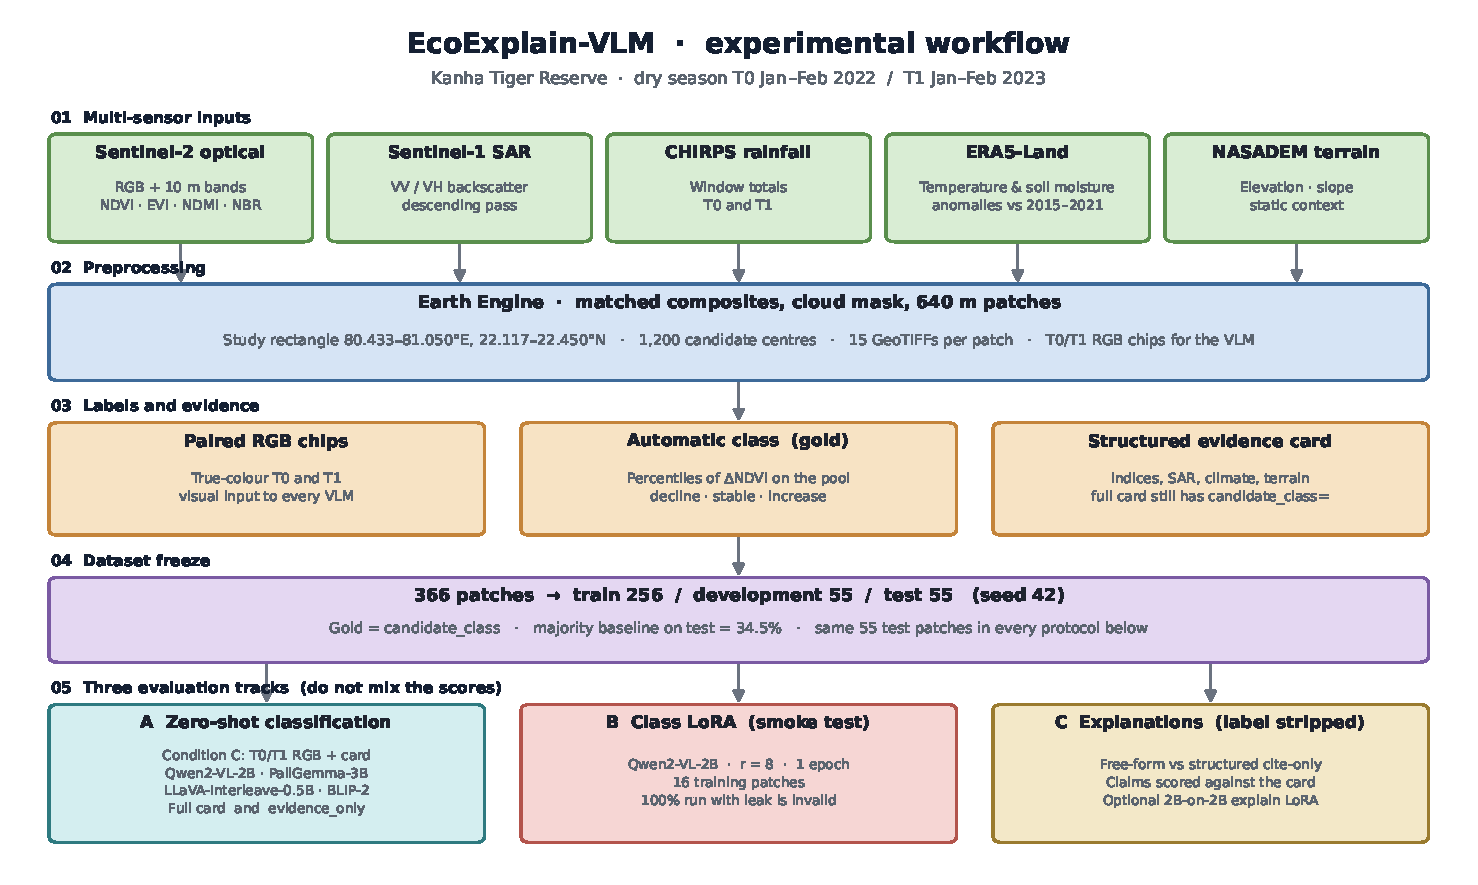
\includegraphics[width=\textwidth]{fig_workflow.pdf}
\caption{End-to-end EcoExplain-VLM workflow. Multi-sensor dry-season
stacks are composited in Earth Engine, labelled by $\Delta$NDVI
percentiles, packed as RGB chips plus an evidence card, and frozen
into a 256/55/55 split. Evaluation then follows three tracks that
must not be pooled: (A)~zero-shot classification on the full card
and after stripping \texttt{candidate\_class=}; (B)~a 16-example
class LoRA smoke test; (C)~explanations with the label removed
(free-form, structured cite-only, and optional explanation LoRA).}
\label{fig:workflow}
\end{figure*}

Figure~\ref{fig:workflow} is the pipeline used in this paper.

\begin{enumerate}
\item Export multi-sensor stacks and RGB chips from Earth Engine.
\item Attach automatic labels and evidence cards; split 256/55/55.
\item Zero-shot Condition~C on four models (full card).
\item Ablate the summary line (\texttt{evidence\_only}).
\item Class LoRA smoke test (16 rows) on Qwen2-VL-2B.
\item Generate explanations with the label removed; score claims.
\item Compare free-form vs.\ structured cite-only prompts.
\item Optional: filter self-generations and run explanation LoRA.
\end{enumerate}

All four models see the same 55 test patches. Development data are
used only for prompt wording and for the closed-set bias probe, never
to pick the headline accuracy after looking at test.

% ============================================================
% 3. RESULTS AND DISCUSSION
% ============================================================

\section{Results and Discussion}

\subsection{Dataset Characteristics}

Table~\ref{tab:data} summarises the benchmark. NDVI, NBR, NDMI and
EVI changes co-move (correlations of $\Delta$NDVI with $\Delta$NBR,
$\Delta$NDMI and $\Delta$EVI are 0.80, 0.77 and 0.78). Rainfall falls
from 69.1\,mm in the 2022 window to 25.1\,mm in 2023; temperature
anomaly moves from $-1.52^\circ\mathrm{C}$ to $+0.88^\circ\mathrm{C}$;
soil-moisture anomaly from $+0.024$ to $-0.043$. Mean VV/VH changes
are $-0.47$ / $-0.48$\,dB. The optical and climate fields therefore
point, on average, toward a drier, slightly browner dry season, which
is why ``increase'' is a relative rank and why many increase patches
have $\Delta$ near zero.

\begin{table}[t]
\centering
\small
\begin{tabular}{lr}
\toprule
Quantity & Value \\
\midrule
Study rectangle & 2,350.7\,km$^2$ \\
Candidate pool / final patches & 1,200 / 366 \\
decline / stable / increase & 120 / 124 / 122 \\
Train / development / test & 256 / 55 / 55 \\
Test class counts (d / s / i) & 18 / 18 / 19 \\
Majority baseline (test) & 34.5\% \\
Human agreement (19 patches) & 8/19 (42\%) \\
Mean $\Delta$NDVI (s.d.) & $-0.016$ (0.027) \\
Patches with $|\Delta\mathrm{NDVI}|\ge 0.05$ & 34 \\
\bottomrule
\end{tabular}
\caption{EcoExplain-VLM dataset facts. Labels are NDVI-change ranks
inside this region and year pair.}
\label{tab:data}
\end{table}

\subsection{Zero-Shot Model Performance}

Table~\ref{tab:zeroshot} reports generative zero-shot accuracy on the
55-patch test set. Qwen2-VL-2B is the only model clearly above the
majority baseline (56.4\%, 31/55; Wilson interval roughly 43--69\%).
PaliGemma-3B, LLaVA-Interleave-0.5B and BLIP-2 OPT-2.7B occupy
32.7--36.4\%, consistent with chance plus weak class bias.

\begin{table}[t]
\centering
\small
\begin{tabular}{lcc}
\toprule
Model & Acc.\ (full card) & vs.\ majority \\
\midrule
Majority class (increase) & 34.5\% & --- \\
Qwen2-VL-2B & \textbf{56.4\%} & $+$21.9 \\
PaliGemma-3B & 32.7--36.4\% & $\approx 0$ \\
LLaVA-Interleave-0.5B & 32.7--36.4\% & $\approx 0$ \\
BLIP-2 OPT-2.7B & 32.7--36.4\% & $\approx 0$ \\
\midrule
Same three, card w/o label line & 32.7--36.4\% & $\approx 0$ \\
\bottomrule
\end{tabular}
\caption{Zero-shot classification, $n=55$. Headline figure is
Qwen2-VL-2B at 56.4\% on the full evidence card. The 32.7--36.4\%
band is chance-level. Removing the pipeline summary line leaves the
three retested models in that band.}
\label{tab:zeroshot}
\end{table}

Two observations follow. First, parameter count in this 0.5--3B
range is not predictive: the 2B Qwen checkpoint outperforms the 3B
PaliGemma checkpoint on this card format. Second, the full-card
condition is not a pure vision test. The models that fail to use the
leaked line stay at chance; the model that exceeds chance may be
reading that line, the indices, the images, or a mixture. The
\texttt{evidence\_only} ablation is the fairer estimate of ``can the
model classify from sensors and text facts,'' and it is not above
chance for the three models we have scored that way.

\subsection{Effect of Fine-Tuning}

Class LoRA on 16 patches and one epoch raises Qwen2-VL-2B from 56.4\%
to \textbf{67.3\%} (Table~\ref{tab:lora}). With $n=55$, the Wilson
intervals of 56.4\% and 67.3\% overlap; the gain is a smoke-test
signal, not a powered comparison. We do not report the 100\% LoRA
run: it was trained with the leaked \texttt{candidate\_class=} line
and is consistent with copying the answer.

\begin{table}[t]
\centering
\small
\begin{tabular}{lcc}
\toprule
Run & Train rows & Test acc. \\
\midrule
Zero-shot Qwen2-VL-2B (full card) & 0 & 56.4\% \\
Class LoRA, 1 epoch & 16 & 67.3\% \\
Class LoRA with label leak & --- & 100\% (invalid) \\
\midrule
Explain LoRA (label-free card) & 16 of 28 & 61.8\% \\
\quad claim correctness & --- & 50.5\% \\
\bottomrule
\end{tabular}
\caption{LoRA results for Qwen2-VL-2B. Class 67.3\% and explain
61.8\% are different tasks and must not be averaged or stacked.}
\label{tab:lora}
\end{table}

Explanation LoRA is a different task (Section~\ref{sec:expl}).
Teacher quality is the bottleneck: only 28/256 training generations
passed the filter (gold class, $\ge 2$ claims, 100\% faithful).
Training on 16 of those rows yields 61.8\% class accuracy in
explanation mode---higher than chance, lower than the class smoke
test---and 50.5\% claim correctness, which is worse than structured
zero-shot citing. Self-distillation of the 2B model does not, on
this evidence, teach faithful explanation.

\subsection{Error Analysis}

Errors concentrate where the label is a weak rank. Increase patches
with $\Delta$ near zero are easy to call stable; decline patches
near $q_{15}$ sit next to stable patches after the second-batch
percentile shift. Cards whose prose NDVI trend disagrees with
\texttt{candidate\_class} (108/366) are a built-in contradiction:
a model that ``reads the text faithfully'' can still miss the gold
label.

PaliGemma, LLaVA and BLIP-2 often emit a single class token with
little use of the card, or dump a generic vegetation sentence.
Qwen2-VL-2B more often copies numbers from the card, which helps
when those numbers match the rank label and hurts when they do not.
Invalid parses are rare under the closed instruction but not zero;
they are scored as wrong.

Human disagreement (8/19) means a non-trivial fraction of ``errors''
may be label noise rather than model failure. We do not relabel the
test set after seeing model outputs.

\subsection{Explanation Quality}
\label{sec:expl}

Free-form ``explain why'' prompts, with the class line removed,
yield either no checkable numeric claims or claims that contradict
the card (wrong sign of $\Delta$NDVI, invented rainfall, radar
values not in the prompt). That setting is not usable as an audit
trail.

A structured prompt that forbids facts not present in the card, and
asks for a short list of citations plus a class, raises automatic
claim correctness to \textbf{75.8\%} for Qwen2-VL-2B and
\textbf{71.1\%} for LLaVA-Interleave-0.5B (Table~\ref{tab:explain}).
The texts are largely restatements of the supplied rows. High claim
correctness here means ``the model did not invent numbers,'' not
``the model reasoned about disturbance.'' This is the intended
conservative reading \citep{jacovi2020,turpin2023}.

\begin{table}[t]
\centering
\small
\begin{tabular}{lcc}
\toprule
Setting & Class acc. & Claim correct \\
\midrule
Free-form explain (label off) & low / unstable & few or conflicting \\
Structured cite-only, Qwen2-VL-2B & --- & 75.8\% \\
Structured cite-only, LLaVA-0.5B & --- & 71.1\% \\
Explain LoRA, Qwen2-VL-2B & 61.8\% & 50.5\% \\
\bottomrule
\end{tabular}
\caption{Explanation protocol, label stripped from the card.
Structured prompting is the only setting in which most numeric
claims match the evidence.}
\label{tab:explain}
\end{table}

\subsection{Comparison with Existing Approaches}

Pixel and segment change detectors \citep{hansen2013,kennedy2010,zhu2014,daudt2018}
optimise map accuracy, not a three-class patch rank plus a sentence.
They remain the correct tool if the goal is a wall-to-wall
disturbance map. EcoExplain-VLM asks a different question: whether
a general VLM can consume the \emph{same} multi-sensor packet a
human analyst would see.

Remote-sensing VLMs \citep{kuckreja2024} are trained on overhead
imagery and spatial referring expressions. They are a natural next
baseline; they are not evaluated in this paper because the present
compute envelope was 0.5--3B general checkpoints on a 16\,GB
cluster queue. CLIP-style encoders \citep{radford2021} could score
the RGB pair without generation; they would not produce the
justification the benchmark is named for.

Against a majority baseline, only Qwen2-VL-2B under the full card
clears a meaningful margin. Against a leak-free card, the small
models tested here do not. That comparison, not a comparison to
LandTrendr F1, is the one this dataset supports.

% ============================================================
% 4. LIMITATIONS AND FUTURE DIRECTIONS
% ============================================================

\section{Limitations and Future Directions}

\textbf{Labels.} Classes are percentiles of one-year dry-season NDVI
change, not validated disturbance, degradation or recovery. Absolute
change is small. Human agreement on 19 patches is 42\%. An expert
audit and a second annotator are required before any management use.

\textbf{Leak.} The production evidence card contains
\texttt{candidate\_class=}. Headline 56.4\% and class LoRA 67.3\%
use that card. Leak-free numbers should be the default in follow-on
work; the codebase now supports an \texttt{evidence\_only} view.

\textbf{Split.} Random stratified splitting does not block spatial
leakage \citep{ploton2020}. A block split by sub-landscape should be
added as a second official test.

\textbf{Models.} Results are for four small open VLMs. They do not
license claims about GPT-class or remote-sensing-pretrained models.
PaliGemma access is gated; BLIP-2 is a different architecture family
and is a weak generative classifier in this protocol.

\textbf{Explanations.} Automatic claim matching can miss paraphrases
and can reward copying. Structured 75.8\% / 71.1\% correctness is
not human-judged faithfulness. Explanation LoRA used a 2B teacher on
itself (28/256 kept); a stronger frozen teacher is the obvious next
experiment, subject to disk and memory limits.

\textbf{Geography.} One reserve, one year pair, one season. External
validity to other parks, wet-season composites, or fire-year extremes
is unknown.

Future work that would change the scientific picture, rather than
add leaderboard rows: (i)~leak-free evaluation as the only primary
table; (ii)~spatial block test; (iii)~expert labels on the full 366
or a powered subsample; (iv)~LoRA on the full 256 with early
stopping on development, leak stripped; (v)~a larger or
domain-pretrained VLM under the same cards.

% ============================================================
% 5. CONCLUSIONS
% ============================================================

\section{Conclusions}

EcoExplain-VLM packages 366 Kanha patches, matched 2022/2023
dry-season Sentinel-2 and Sentinel-1 chips, climate and terrain
context, and a three-class rank label into a reproducible VLM
benchmark. On the 55-patch test set, Qwen2-VL-2B reaches 56.4\%
zero-shot accuracy on the full evidence card; PaliGemma-3B,
LLaVA-Interleave-0.5B and BLIP-2 OPT-2.7B remain at 32.7--36.4\%,
indistinguishable from the 34.5\% majority baseline. A 16-example
class LoRA of Qwen2-VL-2B reaches 67.3\%. Those two figures are not
leak-free. With the candidate-class line removed, the three models
retested stay at chance. Structured cite-only prompting is what
makes explanations numerically consistent (75.8\% and 71.1\% claim
correctness); free-form text does not. A 16-row explanation LoRA
gives 61.8\% class accuracy and 50.5\% correct claims and should
not be cited as an improvement on 56.4\% or 67.3\%.

Small open VLMs, as evaluated here, are not a substitute for
spectral change detection in Kanha. They can, under a constrained
prompt, repeat the facts they are given. The benchmark's use is to
make that limitation measurable and to give larger or
domain-adapted models a fixed test they cannot pass by reading
\texttt{candidate\_class=} off the card.

% ============================================================
% ACKNOWLEDGEMENTS
% ============================================================

\section*{Acknowledgements}

The authors thank the Lab for Spatial Informatics, International
Institute of Information Technology Hyderabad, and the Ada compute
facility used for VLM inference and LoRA. Sentinel-1/2 data are
provided by ESA Copernicus; CHIRPS, ERA5-Land and NASADEM are
used under their respective open licences. Kanha Tiger Reserve is
administered by the Madhya Pradesh Forest Department and the
National Tiger Conservation Authority; this study uses satellite
and reanalysis layers only and is not an official reserve
assessment.

% ============================================================
% REFERENCES
% ============================================================

\bibliography{references}

% ============================================================
% APPENDIX
% ============================================================

\clearpage
\appendix

\section{Additional Experimental Details}

\subsection{Fine-Tuning Configuration}

Class LoRA and explanation LoRA both use Qwen2-VL-2B-Instruct,
rank $r=8$, $\alpha=16$, targeting attention projection modules,
AdamW, learning rate on the order of $10^{-4}$, batch size constrained
by a 16\,GB GPU-memory QoS cap, and one epoch. The class smoke test
and the explanation run each use 16 training rows (the explanation
pool after filtering is 28 rows; 16 are taken to match the class
cap). Mixed-precision inference uses the Hugging Face Transformers
stack. Hugging Face Xet downloads were disabled on the cluster after
writer-channel failures; a 7B teacher download was aborted after a
disk-quota error (OSError 122), which is why the explanation teacher
is the 2B model itself.

The invalid 100\% class LoRA is documented only as a negative
control: training and evaluating with \texttt{candidate\_class=}
still in the prompt is sufficient to explain a perfect score and is
not a measure of visual or spectral understanding.

\subsection{Prompt and Output Parsing}

Classification prompt (abridged): two images (T0, T1), then the
evidence card, then ``Reply with exactly one token:
\texttt{stable}, \texttt{decline}, or \texttt{increase}.''
The parser lowercases the completion, strips punctuation, and
accepts the first exact class word; otherwise the item is wrong.

Leak-free prompt uses the same instruction after deleting lines
that match \texttt{candidate\_class=} and equivalent summary
phrases. Structured explanation prompt requires: (1)~only cite
quantities present in the card; (2)~list them as short claims;
(3)~end with a class word. Free-form explanation prompt asks for
a paragraph of reasoning without that citation constraint.

Teacher filtering for explanation LoRA keeps a generation only if
parsed class equals gold, at least two numeric claims are extracted,
and every extracted claim matches the card. That filter passed
28/256 training rows.

\subsection{Additional Results}

Test size $n=55$ implies wide intervals: 31/55 (56.4\%) and 37/55
(67.3\%) are compatible with a surprisingly large range of true
accuracies. Per-class recalls for Qwen2-VL-2B zero-shot follow the
rank structure (stronger on decline than on near-zero increase)
but are not stable enough, given $n\approx 18$ per class, to
support a fine-grained error taxonomy. Closed-set LLaVA at 60\%
after development bias correction is recorded as a probe, not as a
primary number. No result in this appendix overrides
Tables~\ref{tab:zeroshot}--\ref{tab:explain}.

\end{document}
